\documentclass{article}[12pt]
\usepackage[utf8]{inputenc}
\usepackage[margin=1in]{geometry}
\usepackage{amsrefs,url,template,algorithm,algorithmic,multicol}


\title{\Large{Pop the Balloon}\medskip\\\large A CS175 Final Project}
\author{Annie Zhu\quad \href{mailto:szhu@college.harvard.edu}{szhu@college.harvard.edu}}
\date{May 2021} 

\begin{document}
\maketitle

\section{Project description}

In this project,\footnote{Github repo \href{https://github.com/asyz8/pop-the-balloon/}{\color{blue} here}.} we have designed a simple arrow shooting game, where the goal is to hit the balloons by throwing an arrow. The code is completed in OpenGL and extensively modified from the last few assignments in CS175 Spring 2021 taught by Prof. Steven Gortler.

All objects including the \texttt{g\_skyNode} viewer are confined within a small room, which is divided into two spaces by a translucent red screen. The player is confined to the space in front of the screen (call it space $A$) and can manipulate an arrow, changing its direction and location within space $A$. When ready, the player can specify the position, orientation and starting speed by which the arrow is launched. The arrow will then fly through the space and stop when it hits a wall, at which point we start the round again. Also confined to space $A$ are two lights, which can be moved around. 

On the other side of the screen (space $B$), we can randomly generate balloons, which will either be stationary or elastically bounce around in the room. When the arrow is launched, it may hit some of the balloons, in which case they get popped, and the player gets $10$ points. The trajectory of the arrow is only affected by gravity and nothing else, and it will only terminate when it hits one of the six boundaries of the room. 

\section{User's guide}

\subsection{The interface}
For set-up, run the make file.
Upon running the executable (\texttt{main} or \texttt{main.exe}; I use Mac OS), the player will see the red screen and the small blue arrow. See \cref{fig:init}. By default, the player manipulates the sky camera in orbit mode, but they can also use the picker to choose the arrow or one of the two light globes. They can also move to the other side, in which case the arrow, the walls and the light globes remain visible. In particular, pressing [V] allows the user to switch between the sky camera view, the tip-of-arrow view and the straddled-on-arrow view. The latter two can help a lot with aiming and can also be fun to watch once the arrow is launched. In the second and third view, the arrow can only be translated but not rotated. 

\subsection{Game play}

The player should start by generating some balloons in  by pressing [G] for one balloon or [F] for twenty at a time. The balloons are immobile by default but can be switched between paused and in motion by pressing [N]. When generated, each balloon is at a uniformly random location within section $B$ and travels in a spherically uniformly random direction with a set velocity that is shared by all balloons. The balloons cannot be manipulated by the picker. 
When encountering either one of the five walls or the red screen, the balloon gets bounced off elastically. The balloons are not affected by gravity, as we can assumed they are simply filled with air and the skin is negligible.

When the ready, the player can try launching the arrow. This is done in two stages. In stage 1, the player uses the picker to select the arrow and manipulate it with arcball. When satisfied, they can press [L] to enter \emph{launch mode}, where the picker gets frozen, and all vertical mouse dragging the screen gets interpreted as setting the launch velocity of the arrow. Dragging up speeds up the arrow and dragging down slows it down. The player can press [Q] in this mode to query for the certain starting velocity, though I would love to find a better way of visualizing it if given more time. No matter the orientation, the arrow always launches in the direction its tip is pointing. 

When all is properly adjusted, the player can press [A] to launch the arrow in \emph{animation mode}. It is recommended to try the other two viewing modes. See \cref{fig:view} for examples. The arrow cannot be picked or reset during this process, though of course the sky camera and the two light globes can still be moved. The current round terminates after the arrow hits one of the six walls. The program is put to sleep for three seconds, after which a new round starts. The arrow and the sky camera are reset, though the rest of the configuration (generated, unpopped balloons and the two lights) stay the same. The player score from the total tally of all rounds is reported and also not cleared. 
\begin{figure}[b]
    \centering
    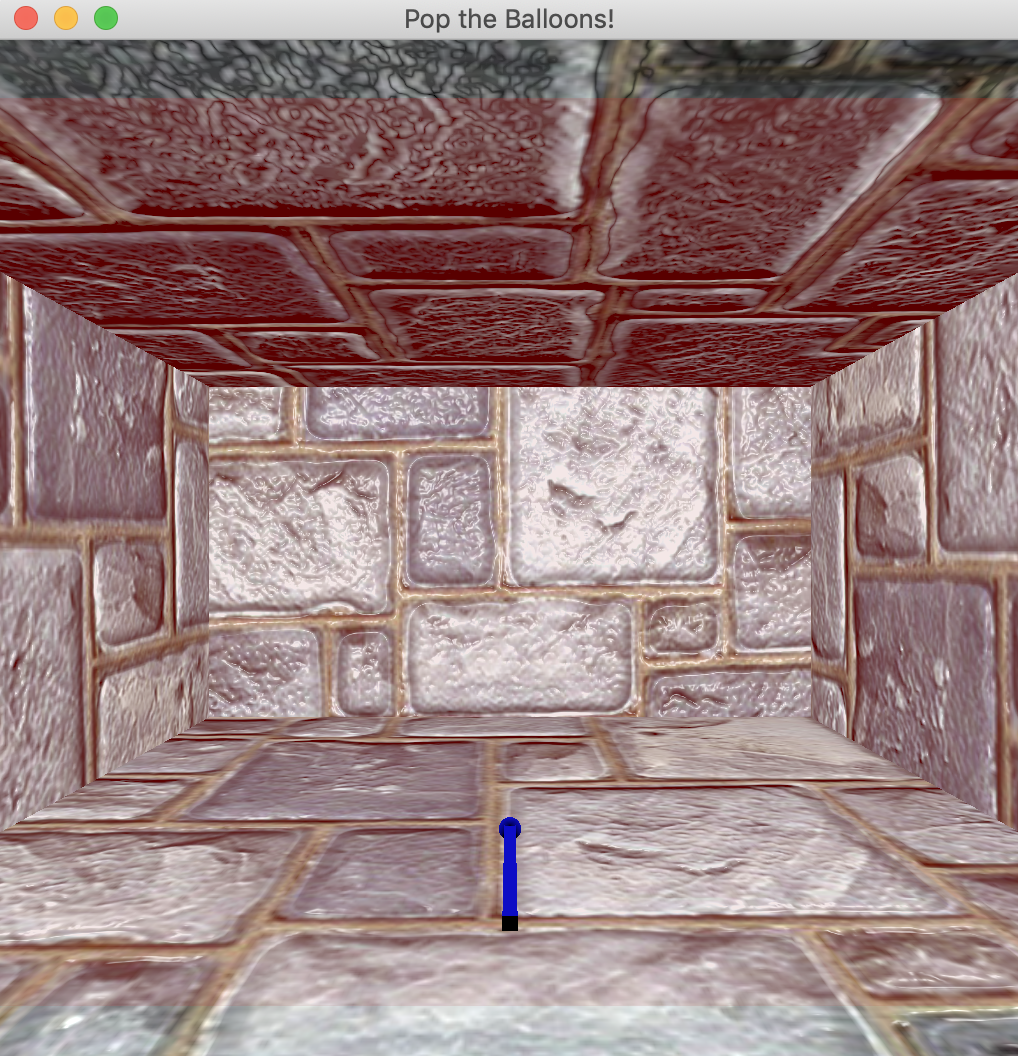
\includegraphics[width=.47\textwidth]{init-a.png}
    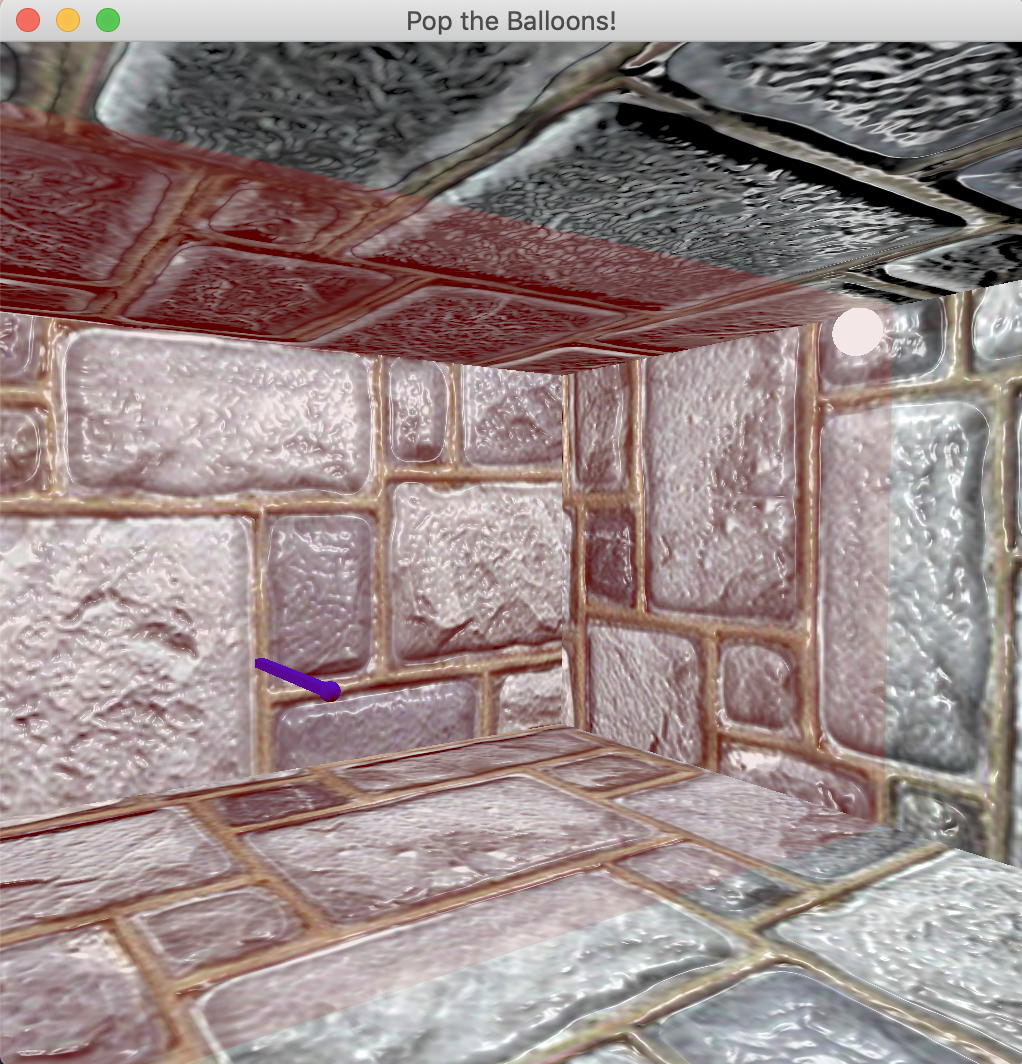
\includegraphics[width=.47\textwidth]{init-b.png}
    \caption{Initial view from both sides of the red screen. The blue arrow is visible in both, though enlarged for higher visibility in the one on the right. 
    \label{fig:init}}
\end{figure}

\begin{figure}[b]
    \centering
    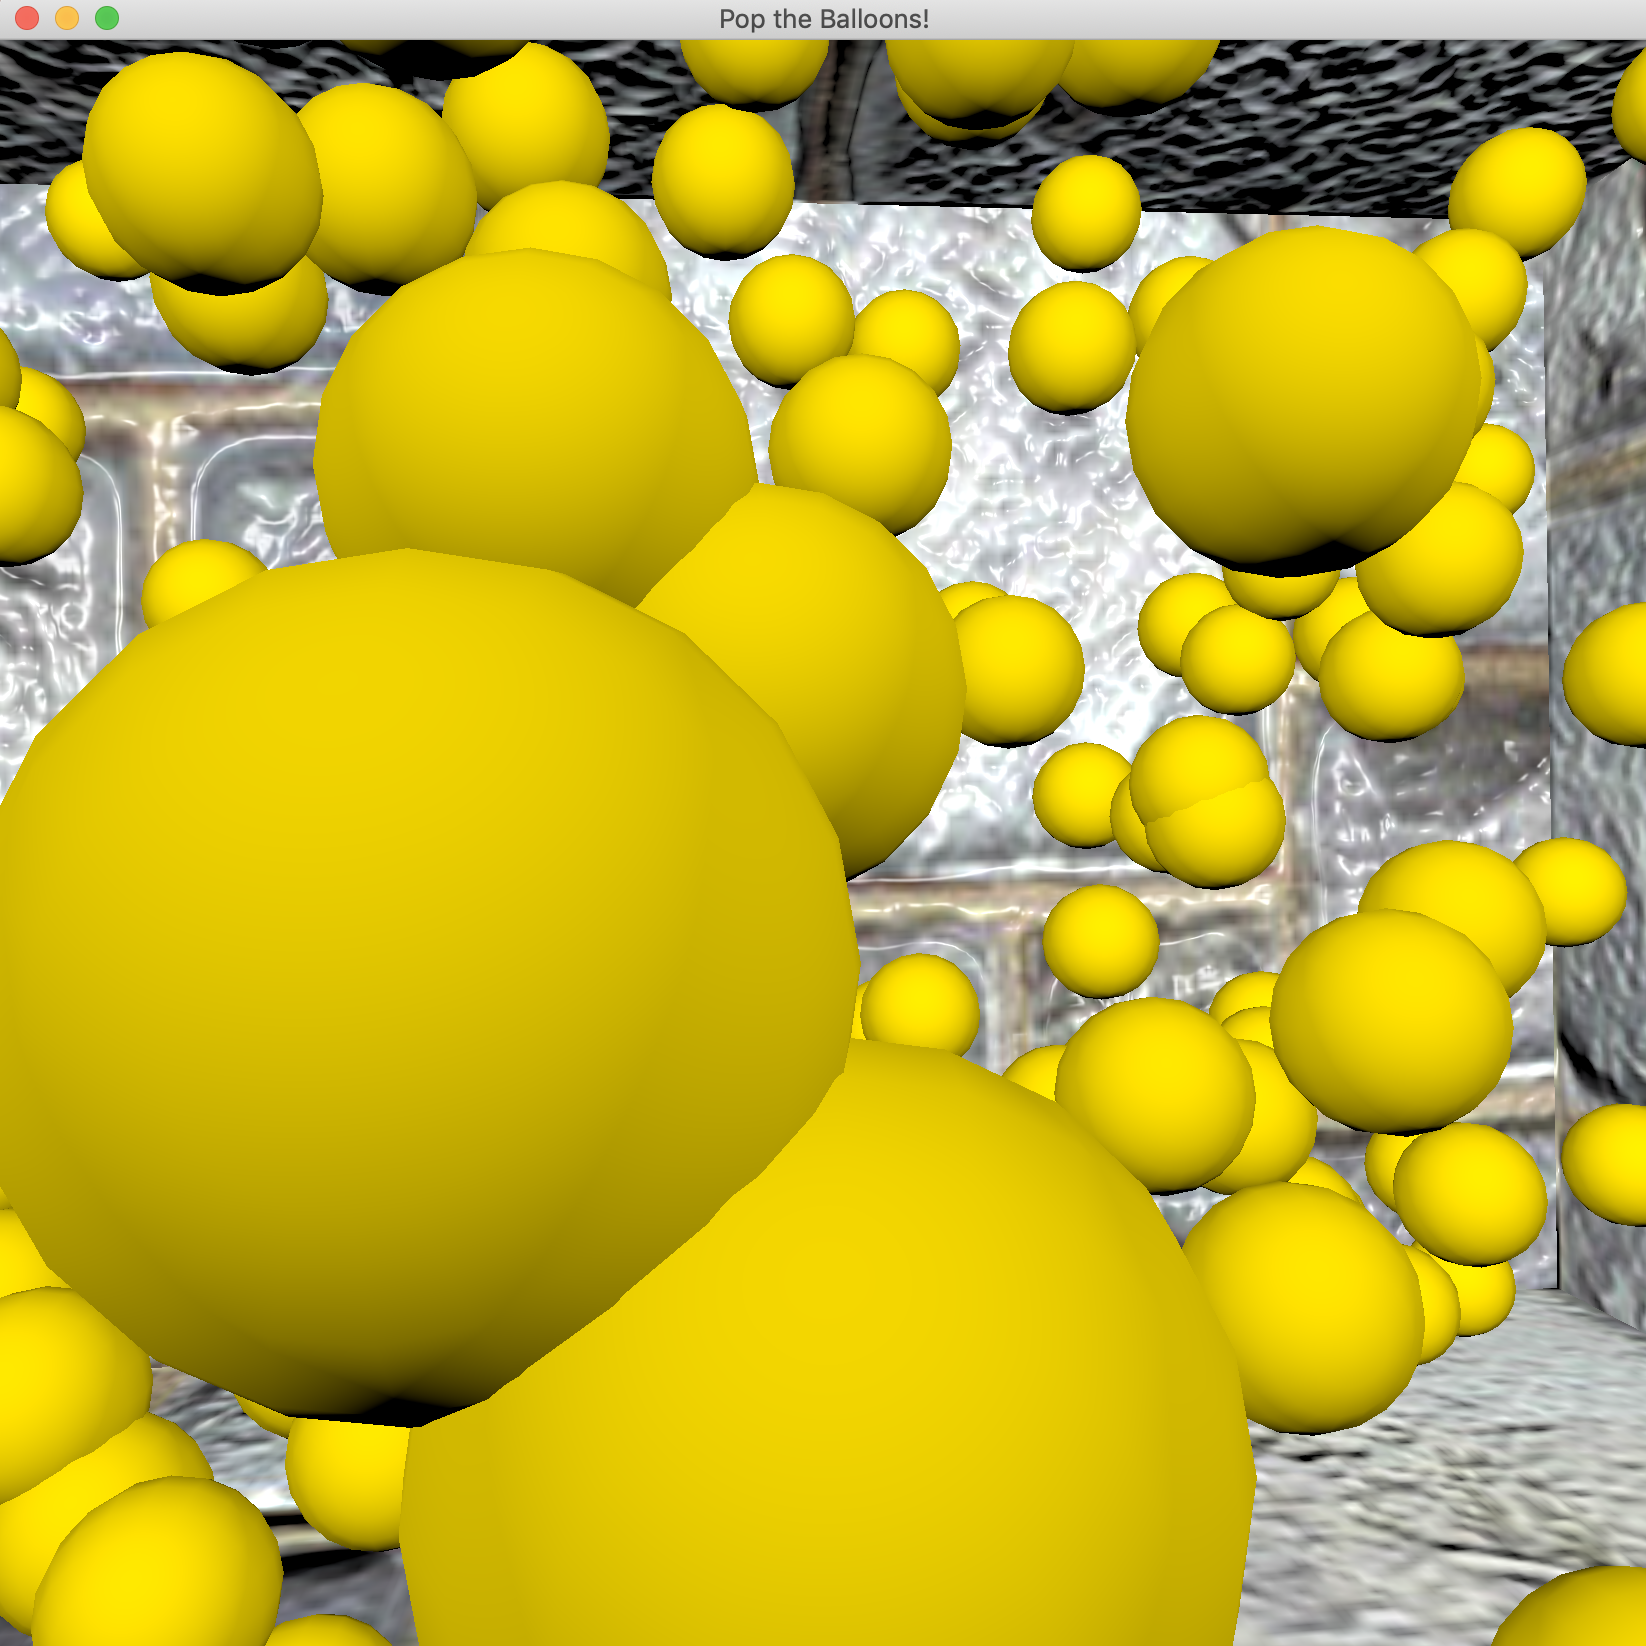
\includegraphics[width=.47\textwidth]{flight-a.png}
    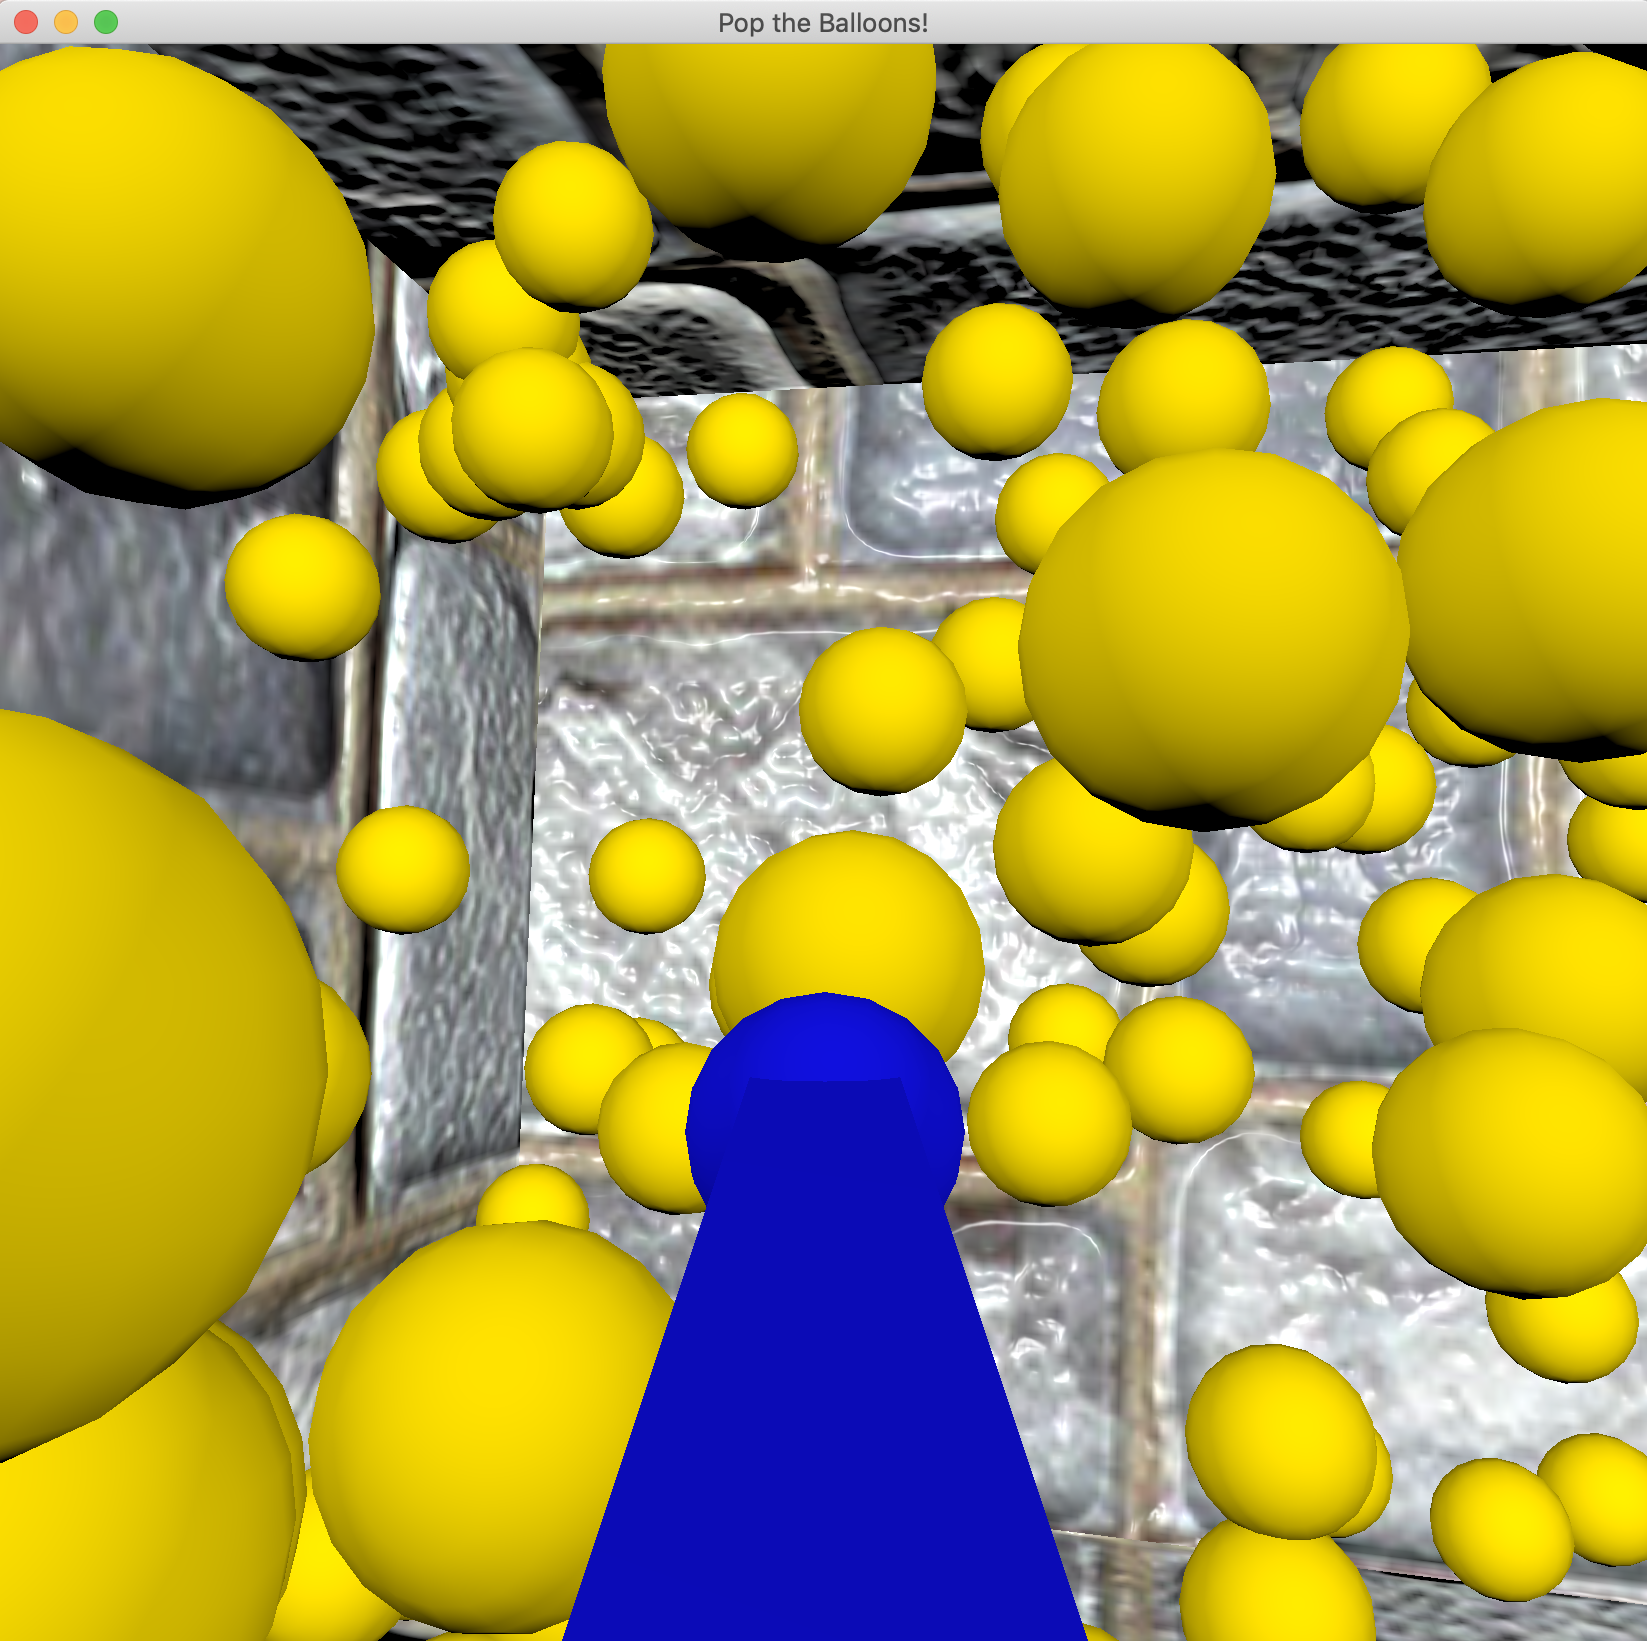
\includegraphics[width=.47\textwidth]{flight-b.png}
    \caption{Tip-of-arrow and straddled-on-arrow view in mid-flight. 
    \label{fig:view}}
\end{figure}

For a summary of all the commands, see \cref{tab:appendix} in the Appendix. 

\subsection{Parameters}

For better user experiences, one can shrink or enlarge the arrow by pressing [-] and [+] within a certain range. The arrow is comprised of a long rod with ratio $1:1:20$ and a spherical tip centered at the tip of the arrow and whose radius is equal to the width of the rod. The definition of piercing a balloon is such that the spherical tip intersects with the balloon, so it will be much easier to hit a balloon with a larger arrow. Similarly, we can use [$\uparrow$] and [$\downarrow$] to enlarge or shrink the balloons, though they cannot exceed the size of the room or become so small that I deem invisible. 

We can also use [$\leftarrow$] and [$\rightarrow$] to decrement or increment the speed of the balloons within a certain range. This only affects the norm of the velocity vector (hence \emph{speed}) but not its direction. The speed is capped to prevent motion sickness from watching the simulation (don't ask me how I know). 

\section{Challenges \& next steps}
Here are some code design choices that I found interesting and worth mentioning. 

\subsection{Limited motion}
Previously in the homework assignments, all objects and agents are virtually in free space. Here we have confined them to a small room. My solution is to clamp the translation component of all objects to within the space they belong. This is done at the end of the motion function, before the \texttt{rbt} gets updated.

My implementation is not perfect though. Right now I have set a default \texttt{g\_movementBuffer =1.0} and made sure that the centers of the spherical lights and the sky camera do not get closer than that to any of the walls. The balloons are also constrained with the buffer set equal to their radius. This method doesn't work for any object that is not spherical. For instance, I have set the buffer as half the arrow length for the arrow, but this is definitely an overshoot. It would be interesting to develop a way of calculating the convex hull of all children in the scenegraph of a node, which would prevent all kinds of shapes from poking through the walls or the screen when that is not intended. 

\subsection{Balloon motion}
The balloons bounce off the walls in full elastic collisions. This is my default implementation. Other possible ideas include some kind of damping, or perhaps put the balloons under the effect of gravity and disappear once they touch the ground. This could make the game more difficult by forcing the players to shoot the balloons with a time constraint

Meanwhile, overlapping of the balloons is allowed because collision is difficult to model physically, though it can therefore be a goal of future work. I am simply not very familiar with the physics by which this works. 

Another direction of future work is to consider ``intelligent balloons.'' Right now, these are just inanimate objects that move at random specified directions. It would be interesting to consider intelligent beings (say \emph{birds}) who can change direction based on the behavior of the rest of the flock. For instance, we can consider BOID motion and in particular the separation component, which would make collision less likely and also make the game harder because the player will hit fewer targets in one launch of the arrow. 

\subsection{Arrow motion}

Figuring out this part took me the most time. We set up the \texttt{rbt} of the arrow such that it is always centered at the origin and elongated in the $z$
-direction, with the tip of the rod at $(0,0,-\texttt{g\_arrowLength}/2)$. This makes setting up the two views very easy, which have translations $(0,0,-\texttt{g\_arrowLength}/2-\texttt{g\_tipRadius})$ (in the code I set this radius equal to the arrow width) and $(0,\texttt{g\_arrowWidth},0)$ (technically it should be half of the width, but then we wouldn't see the arrow itself, so I made the perspective a bit higher), respectively, and identity rotation.  However, this makes rod movement a bit harder. 

We simulate this using time steps, similarly to assignment 9. 
I am making the assumption that at any point in time, the arrow should always be oriented along the tangent line of the trajectory of its center of mass. I think this is a fair assumption for rigid bodies, though I am open to suggestions to corrections. Either way, if $\theta$ is the angle between the old and the new velocity vectors of the arrow, then effectively the $z$-vector also rotates by $\theta$ with respect to an axis $\hat k$ in the $xz$-plane within this time step. 
Moreover, since the only force acting on the arrow is gravity in the $y$-direction, the $xz$-projection of the velocity vector should remain the same, so that $\hat k\perp[v_x,0,v_z]$. We can deduce that $\hat k \propto[-v_z,0,v_x]$ and we just need to nail down the signs, which can be easily accomplished. It now suffices to convert $\hat k$ into the arrow coordinate system and use quaternions to complete the rotation. We can verify that $-\hat z$ in the coordinate system of the arrow is always equal to normalized velocity vector of the arrow (the error is $1e-16$ in my simulations for my hyperparameter setup), so this is indeed correct. 

\subsection{Game design}

It would be interesting to think about how we can make this game engaging. For instance, we can have two colors of balloons, one of which gives points and others are mines that lead to instant gameover when shot. Also, I personally find this game to be quite hard to play and would be open to any advice for making it more accessible. 
\newpage 
\section*{Appendix\label{sec:app}}
\begin{table}[h]
    \centering
    \begin{tabular}{c|l}
\hline Keyboard &   Command  \\\hline
       esc  & Quit program. \\
       H & Open Help menu. \\
       S & Save screenshot as \texttt{out.ppm}.\\
       V & Cycle through three views. \\
       M & Switch between orbit and ego motion for sky camera. \\
       P & Enable picking mode. \\
       G & Generate one balloon. \\
       F & Generate twenty balloons. \\
       R & Reset arrow and sky camera position and orientation.\\
       L & Enable launch mode. Dragging affects launch speed only. \\
       Q & In launch mode, queries launch speed.\\
       A & Enable animation mode. Launch arrow if launch speed is positive. \\
       N & Switch between balloons on pause and in motion.\\
       $\uparrow~(\downarrow)$ & Balloon radius increases (decreases) by $20\%$ unless limit is reached. \\
       $\leftarrow~(\rightarrow)$ & Balloon velocity decreases (increases) by $20\%$ unless limit is reached. \\
       $+~(-)$ & Arrow size increases (decreases) by $20\%$ unless limit is reached. \\
    \end{tabular}
    \caption{A list of all commands.}
    \label{tab:appendix}
\end{table}

\end{document}